% ----------------------------------------------------------------------
%  Set the document class
% ----------------------------------------------------------------------
\documentclass[11pt,a4paper,twoside]{article}

% ----------------------------------------------------------------------
% Define external packages, language, margins, fonts and new commands
% ----------------------------------------------------------------------
%\input{preamble} 
\usepackage[utf8]{inputenc}   % <<<<< Linux
\usepackage[english]{babel} % <<<<< English
\usepackage{notoccite}
\usepackage[skip=0.5\baselineskip]{caption}
\hyphenation{GTKWave}
\usepackage{listings}
\usepackage[all]{nowidow}
\usepackage{amsmath}

%blind text

\usepackage{lipsum}

\usepackage{graphicx}
\graphicspath{ {./} {../../figlib/} }
\def\FontLn{% 16 pt normal
  \usefont{T1}{phv}{m}{n}\fontsize{16pt}{16pt}\selectfont}
\def\FontLb{% 16 pt bold
  \usefont{T1}{phv}{b}{n}\fontsize{16pt}{16pt}\selectfont}
\def\FontMn{% 14 pt normal
  \usefont{T1}{phv}{m}{n}\fontsize{14pt}{14pt}\selectfont}
\def\FontMb{% 14 pt bold
  \usefont{T1}{phv}{b}{n}\fontsize{14pt}{14pt}\selectfont}
\def\FontSn{% 12 pt normal
  \usefont{T1}{phv}{m}{n}\fontsize{12pt}{12pt}\selectfont}

% Use Arial font as default
\renewcommand{\rmdefault}{phv}
\renewcommand{\sfdefault}{phv}

\usepackage{geometry}	
\geometry{verbose,tmargin=2.5cm,bmargin=2.5cm,lmargin=2.5cm,rmargin=2.5cm}

%\usepackage{setspace}
%\renewcommand{\baselinestretch}{1.5}

\usepackage[pdftex]{hyperref} % enhance documents that are to be
                              % output as HTML and PDF
\hypersetup{colorlinks,       % color text of links and anchors,
                              % eliminates borders around links
%            linkcolor=red,    % color for normal internal links
            linkcolor=black,  % color for normal internal links
            anchorcolor=black,% color for anchor text
%            citecolor=green,  % color for bibliographical citations
            citecolor=black,  % color for bibliographical citations
%            filecolor=magenta,% color for URLs which open local files
            filecolor=black,  % color for URLs which open local files
%            menucolor=red,    % color for Acrobat menu items
            menucolor=black,  % color for Acrobat menu items
%            urlcolor=cyan,    % color for linked URLs
            urlcolor=black,   % color for linked URLs
	          bookmarksopen=false,    % don't expand bookmarks
	          bookmarksnumbered=true, % number bookmarks
	          pdftitle={report},
            pdfauthor={Grupo 18},
%            pdfsubject={Thesis Title},
%            pdfkeywords={Thesis Keywords},
            pdfstartview=FitV,
            pdfdisplaydoctitle=true}

\usepackage[numbers,sort&compress]{natbib} % <<<<< References in numbered list [1],[2],...
\usepackage{subcaption} 
\usepackage{mdframed}
\usepackage{indentfirst}


%%%%%%%%%%%%%%%%%%%%%%%%%%%%%%%%%%%%%%%%%%%%%%%%%%%%%%%%%%%%%%%%%%%%%%%%
%     Begin Document                                                   %
%%%%%%%%%%%%%%%%%%%%%%%%%%%%%%%%%%%%%%%%%%%%%%%%%%%%%%%%%%%%%%%%%%%%%%%%


\begin{document}

% Set plain page style (no headers, footer with centered page number)
\pagestyle{plain}

% Set roman numbering (i,ii,...) before the start of chapters
%\pagenumbering{roman}

% ----------------------------------------------------------------------
%  Cover page
% ----------------------------------------------------------------------
%%%%%%%%%%%%%%%%%%%%%%%%%%%%%%%%%%%%%%%%%%%%%%%%%%%%%%%%%%%%%%%%%%%%%%%%
%                                                                      %
%     File: Thesis_FrontCover.tex                                      %
%     Tex Master: Thesis.tex                                           %
%                                                                      %
%     Author: Andre C. Marta                                           %
%     Last modified :  2 Jul 2015                                      %
%                                                                      %
%%%%%%%%%%%%%%%%%%%%%%%%%%%%%%%%%%%%%%%%%%%%%%%%%%%%%%%%%%%%%%%%%%%%%%%%

\thispagestyle {empty}

% IST Logo - Signature A
% parameters: bb=llx lly urx ury (bounding box), width=h_length, height=v_length, angle=angle, scale=factor, clip=true/false, draft=true/false. 
\includegraphics[bb=9.5cm 11cm 0cm 0cm,scale=0.29]{IST_A_CMYK_POS}

\begin{center}
%
% Figure (Image or plot)
\vspace{1.0cm}
% height = 50 mm
%\includegraphics[height=50mm]{Figures/Airbus_A350.jpg}

% Title, author and degree
\vspace{1cm}
{\FontLb Circuit Theory and Electronics Fundamentals} \\ % <<<<< EDIT TITLE
\vspace{5cm}
{\FontLn T3 Laboratory Report}\vspace{1cm} \\
\vspace{5cm}
\vspace{1cm}
{\FontSn Guilherme Coelho, Nº 95794} \\
{\FontSn João Bárbara, Nº 95809} \\
{\FontSn João Guedes Félix, Nº 97238} \\
\vspace{1cm}
{\FontSn Aerospace Engineering (MEAer), Técnico, University of Lisbon} \\ % <<<<< EDIT COURSE
\vspace{1cm}
{\FontSn May 5, 2021} \\ % <<<<< EDIT DATE (corresponds to date of oral examination)
%
\end{center}



% ----------------------------------------------------------------------
% Dedication page (optional)
% ----------------------------------------------------------------------
%\input{dedication} 
%\cleardoublepage

% ----------------------------------------------------------------------
%  Acknowledgments (optional)
% ----------------------------------------------------------------------
%\input{acknowledgements}
%\cleardoublepage

% ----------------------------------------------------------------------
%  Abstract (both in English and Portuguese)
% ----------------------------------------------------------------------
%\input{resumo} 
%\cleardoublepage

%\input{abstract} 

% ----------------------------------------------------------------------
%  Table of contents, list of tables, list of figures and nomenclature
% ----------------------------------------------------------------------

% Table of contents
%
\pagebreak
\tableofcontents
\setcounter{page}{1}
% List of tables



% List of figures

\pagebreak

% ----------------------------------------------------------------------
%  Body
% ----------------------------------------------------------------------

\section{Introduction}
\label{sec:introduction}
In this laboratory assignment, we analysed, using both a theoretical and simulation analysis, a Sound Amplifier made of Bipolar Junction Transistors. It was made up of two different stages, a Gain stage, with the goal of having the maximum gain possible, and an output stage, whose goal was to lower the impendance. The circuit is presented in \ref{fig:circuitol3}.

As mentioned above, we analysed the circuit theoreticaly, combining Operating Point, allowing us to derive important values used in the incremental analysis.

Simultaneously, the circuit is analysed by computational simulation tools, via \textit{Ngspice}, and the results are compared to the theoretical results obtained, in Section \ref{sec:analysis}. The conclusions of this study are outlined in Section \ref{sec:conclusion}.

We also used Ngspice to analyse the circuit by computacional tools, and then compared with the results obtained in \ref{sec:analysis}. The results of this comparison are outlined in \ref{sec:conclusion}.



\begin{figure}[h] \centering
\includegraphics[width=1\linewidth]{circuitl4.pdf}
\caption{BJT Amplifier}
\label{fig:circuitol4}
\end{figure}

\clearpage


\section{Theoretical and Simulation Analysis}
\label{sec:analysis}

In order to compare \textit{side by side}, we'll discuss the theoretical and simulation analysis at the same time. However, one has to present and analyse the three stages in order to fully understand the simulation. The constants values used are expressed in the table below.

\begin{table}[h]
    \centering
    \begin{tabular}{|l|c|c|}
    \hline
    {\bf Name} & {\bf Value} & {\bf Units} \\ \hline
    $R_1$ & $1000$ & $\Omega$ [Ohms] \\ \hline
    $R_2$ & $1000$ & $\Omega$ [Ohms] \\ \hline
    $R_3$ & $100000$ & $\Omega$ [Ohms] \\ \hline
    $R_4$ & $1000$ & $\Omega$ [Ohms] \\ \hline
    $C_1$ & $220$ & $\eta F$ [$\eta$Farads]\\ \hline
    $C_2$ & $110$ & $\eta F$ [$\eta$Farads] \\ \hline
    \end{tabular}
    \caption[Constants Values]{Constants Values \footnotemark}
    \label{tab:constants}
\end{table}

\footnotetext{Not that the value of $C_1$ reflects two 220 $\eta$F capacitors in series, as seen in Figure \ref{fig:circuitol5}}.

\subsection{High Pass Stage}
\label{subsec:stat}

Firstly, we must discuss the first third of the circuit that was used. 
It is easy to understand that it works as voltage divider,

\begin{equation}
    v_{HP}=v_{R_1}=\frac{R_1}{R1+\frac{1}{j\omega C_1}}v_i
\end{equation}

which can be written as:

\begin{equation}
    A_{HP}=\frac{v_{R_1}}{v_{in}}=\frac{j R_1 \omega C_1}{j R_1 \omega C_1 + 1}
\end{equation}

For high frequencies ($\omega >> 1$), the voltage at the resistor tends to $v_i$ and for low frequencies ($\omega << 1$), it tends to 0.
In reality, this is a simple RC Series circuit, acting as a high pass filter.

A scheme of this circuit is presented below.


\begin{figure}[h]
    \centering
    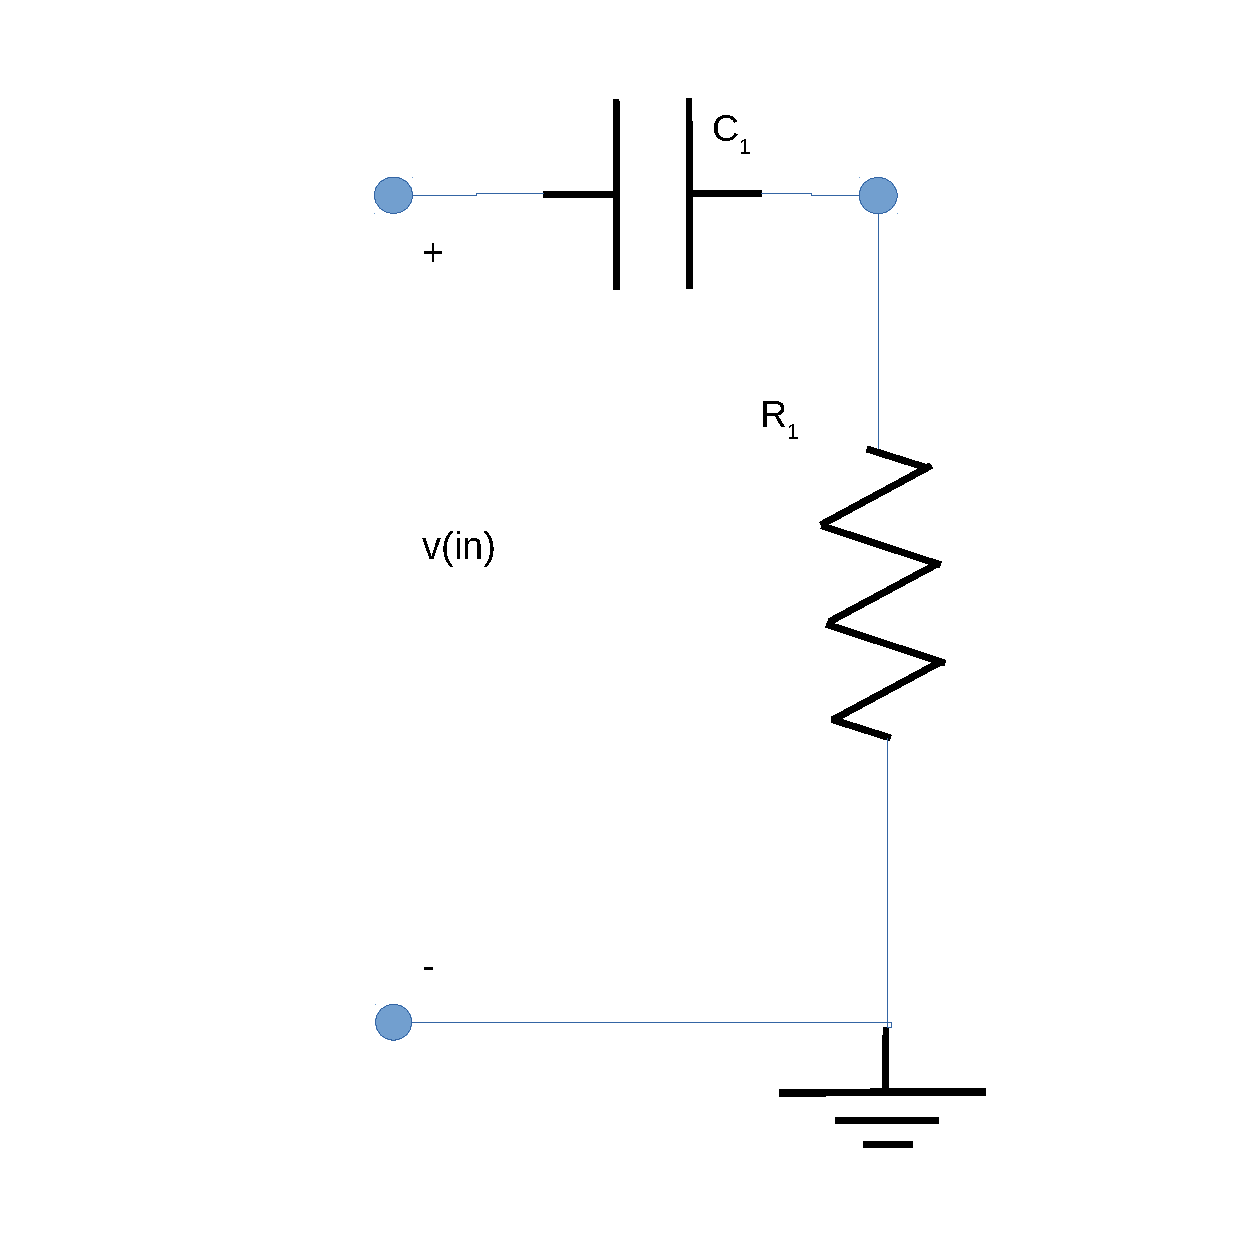
\includegraphics[scale=0.35]{high_pass_l5_old.pdf}
    \caption{High Pass Stage}
    \label{fig:high_pass_stage_old}
\end{figure}

\subsection{Amplification Stage}

In this second stage we have the amplification of the signal. It is where the gain is maximum. This configuration uses a Non-Inverting Amplifier (the + part of the OPAMP is connected to the input \textit{i.e.}, the output of the first stage and the - is connected to the feedback resistors). 
It is worth noticing that, depending on the values of $R_3$ and $R_4$ we can achieve higher or lower gains, hence the gain is given by,

\begin{equation}
    AV_{AMP}=1+\frac{R_3}{R_4}
\end{equation}

A scheme of this stage is presented below, 

\begin{figure}[h]
    \centering
    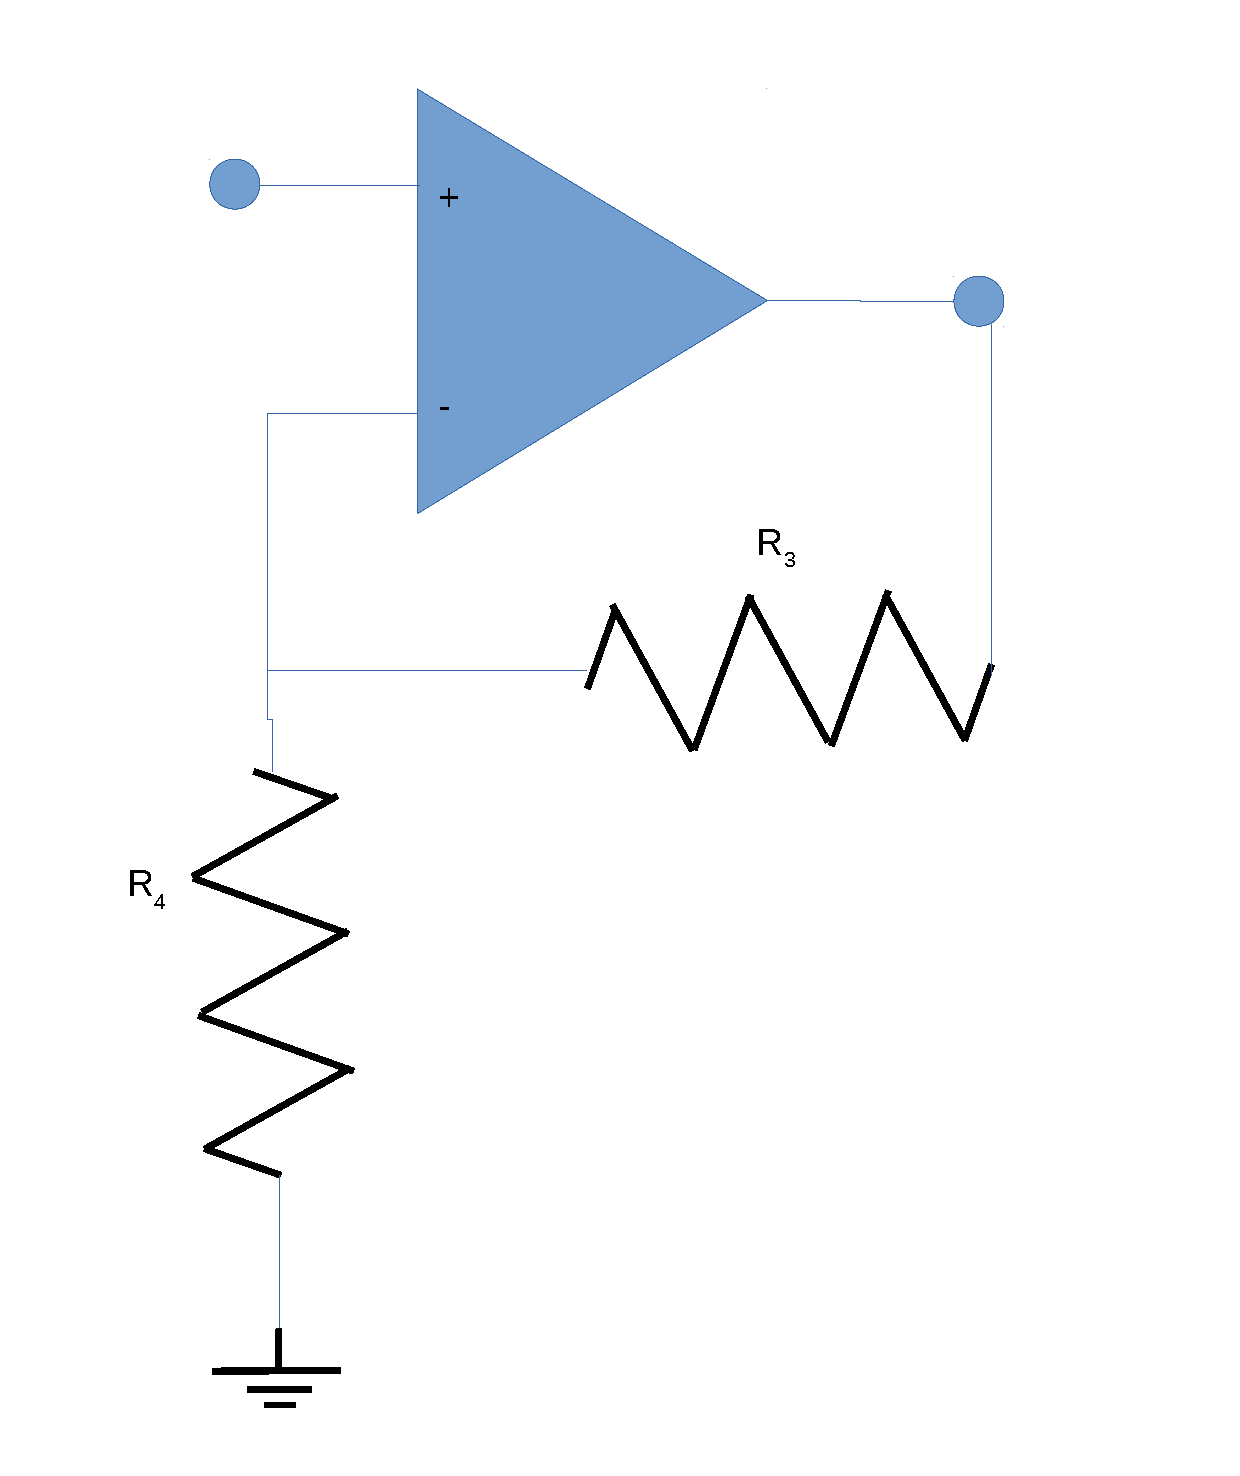
\includegraphics[scale=0.3]{amp_l5_old.pdf}
    \caption{Amplification Stage}
    \label{fig:amp_old}
\end{figure}

\subsection{Low Pass Stage}

In this last stage, we have an analogous circuit to the the High Pass one, except that at this time we are interested in the voltage at the capacitor, instead of the one on the resistor, in order to cut high frequencies.

A scheme of this stage is presented below, in Figure \ref{fig:low_pass}

\begin{figure}[h]
    \centering
    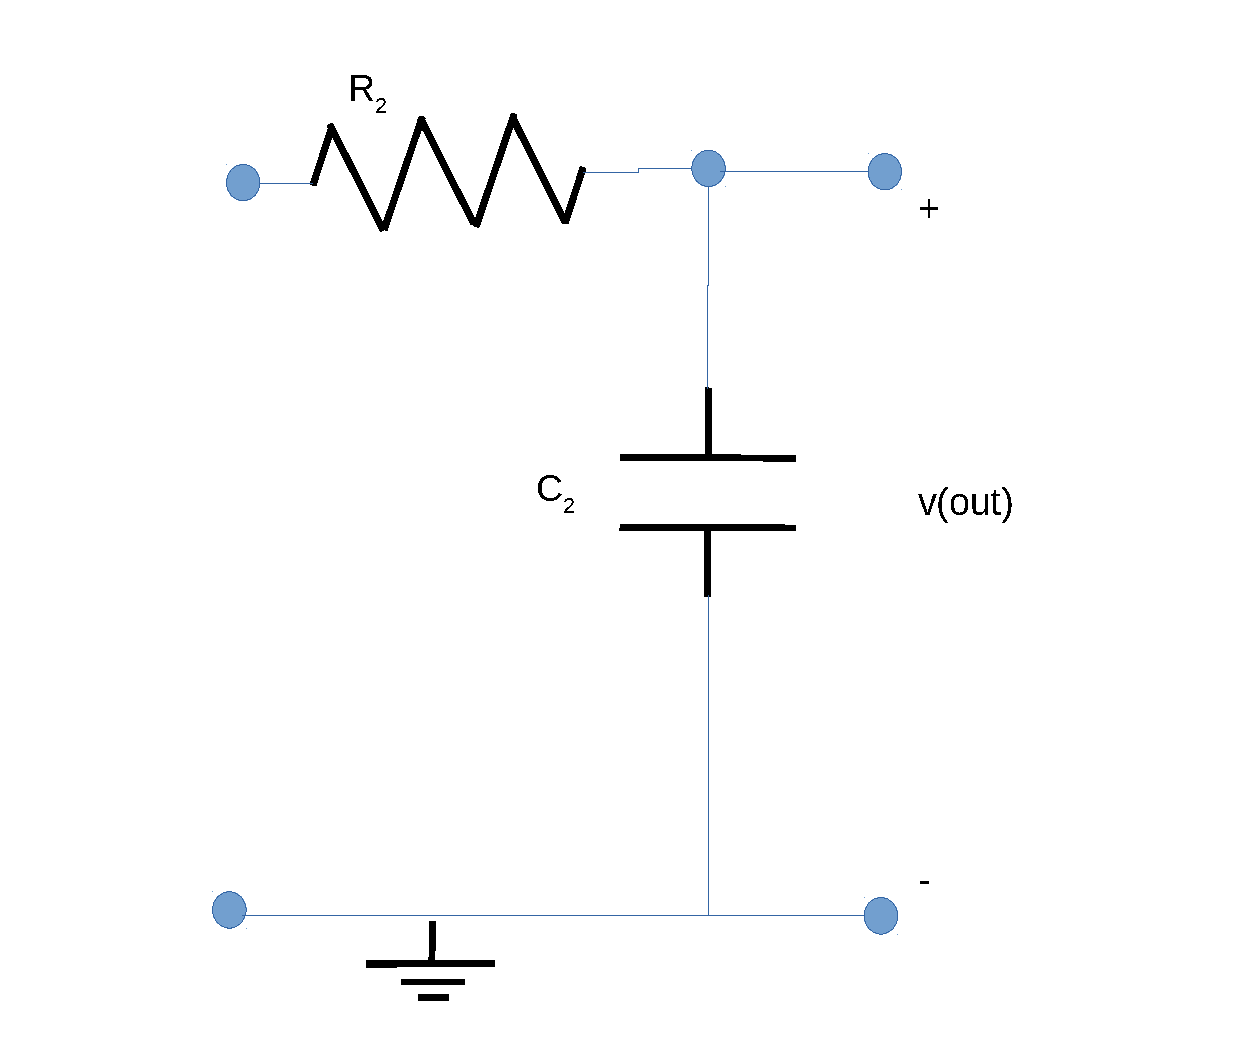
\includegraphics[scale=0.4]{low_pass_l5_old.pdf}
    \caption{Low Pass Stage}
    \label{fig:low_pass}
\end{figure}

By applying the voltage divider law, this time we get:

\begin{equation}
    v_{LP}=\frac{\frac{1}{j \omega C_2}}{\frac{1}{j \omega C_2} + R_2}v_{amp}
\end{equation}

which can be simplified to:

\begin{equation}
    A_{LP}=\frac{v_{LP}}{v_{amp}}=\frac{1}{1 + j \omega C_2 R_2}
\end{equation}

For high frequencies ($\omega >> 1$), the voltage at the capacitor tends to 0 and for low frequencies ($\omega << 1$), it tends to $v_{amp}$.

When combining the three stages, we end up with our Active Pass-band filter as seen in Figure \ref{fig:circuitol5}.

Finally, it is worth noticing that we chose, among other possible options, this circuit's architecture due to its understandable behaviour: a first part blocks low frequencies, a second part amplifies the signal and a last part cuts high frequencies.

\subsection{Theoretical Analysis}
\label{subsec:theo_analysis}

On the Theoretical side, we will evaluate the central frequency ($f_o$), the two impedances: input and output, respectively ($Z_I$ and $Z_O$), as well as the three gains associated with each stage ($AV_{HP}$,$AV_{amp}$ and $AV_{LP}$).

\subsubsection{Central Frequency}

The Central Frequency ($f_o$) is the frequency at the center of the passband of the filter. In this laboratory we want $f_o=\omega_o/2\pi$ to be as close to 1kHz as possible.
\par
As for the mathematical expressions, the Lower Cut-off Frequency ($\omega_L$), the Higher Cut-off Frequency ($\omega_H$) and the Central Frequency are given by,

\begin{equation}
    \omega_L=\frac{1}{R_1C_1} \qquad \omega_H=\frac{1}{R_2C_2} \qquad \omega_o=\sqrt{w_L*w_H}=\sqrt{\frac{1}{R_1C_1R_2C_2}}
\end{equation}

As a remark, if both frequencies, $f_L$ and $f_H$, are equal, $f_o$ is going to be also equal and the passband width is going to be 0 - in the plot, we can see a peak instead of a highland.

The theoretical values of the lower cut-off frequency, the high cut-off frequency, and the central frequency are presented in the table below and will be better analysed and compared in Section \ref{subsec:comparison}.

\begin{table}[h]
   \centering
   \begin{tabular}{|l|c|}
   \hline
   {\bf Name} & {\bf Value [Hz]} \\ \hline
   $f_L$	&	723.431560\\\hline
$f_H$	&	1446.863119\\\hline
$f_O$	&	1023.086723\\\hline

   \end{tabular}
   \caption{Frequencies (Lower, Higher and Central)}
   \label{tab:theo_freq}
\end{table}

\subsubsection{Impedances}

As for the impedances, we have the input and output impedances to be,

\begin{equation}
    Z_I=R_1+Z_{C_1}=R_1+\frac{1}{j\omega C_1} \qquad Z_O=Z_{C_2} || R_2 = \frac{1}{j\omega C_2} || R_2
\end{equation}

Below, we present the values of these impedances, for the asked value of 1kHz,

\begin{table}[h]
    \centering
    \begin{tabular}{|l|c|}
    \hline
    {\bf Name} & {\bf Value [Hz]} \\ \hline
    $Z_{in}$	&	1000.000000-723.431560i\\\hline
$Z_{out}$	&	676.732451-467.723894i\\\hline

   \end{tabular}
   \caption{Impedances}
   \label{tab:theo_imp}
\end{table}

When it comes to the functionality of the circuit, one has to remember that it is important to have a high input impedance (as high as possible) - in order to have a minimum degradation of the input signal. On the other hand, the output impedance needs to be as low as possible, especially when connecting a load to the output of this circuit. Of course, our results regarding the output impedance of the circuit are not satisfactory, however, because of the limitations of the components it was very tough to reduce this. One solution would be to replace $R_2$ with a parallel of several resistances, so that the equivalent resistance would be much less. Another solution would be to add more capacitors in series with $C_2$, decreasing the equivalent reactance seen from a load. However this would be a hard bill to pay because the overall gain would decrease too much below the 40dB wanted, which will be explained in greater detail in the next Section. Adding to this, we were not giving any specific impedance value for the load, but we only can assure good compatibility with very high impedance loads with this specific circuit.  

\subsubsection{Gain}

In order to calculate the total gain ($A_{V}$) we performed a simple multiplication, so that we have $A_{V_{HP}}A_{V_{amp}}A_{V_{LP}}$ (when working with dBs, this multiplication is, in reality, a sum). 

The Transfer Function is given by,

\begin{equation}
    T(s)=\frac{R_1C_1s}{1+R_1C_1s}\bigg(1+\frac{R_3}{R_4}\bigg)\frac{1}{1+R_2C_2s}
\end{equation}

where $s=j\omega+\sigma$ and $\sigma=0$ (for sinusoidal waves).

We can identify $T(s)$ to be the multiplication of $T_i(s)\equiv$ transfer function of the $i-th$ stage. 

When substituting the frequency, $f=\frac{\omega}{2\pi}= 1000 Hz$, we have the results below,

\begin{table}[h]
    \centering
    \begin{tabular}{|l|c|}
    \hline
    {\bf Name} & {\bf Value [dB]} \\ \hline
    $AV_{HP}$	&	-1.828006\\\hline
$AV_{Amp}$	&	40.086427\\\hline
$AV_{LP}$	&	-1.695830\\\hline
$AV$	&	36.562591\\\hline

   \end{tabular}
   \caption{Theoretical Gains}
   \label{tab:theo_gain}
\end{table}

\pagebreak

\subsection{Simulation Analysis}
\label{subsec:sim_analysis}

In regards to the simulation analysis, using the software NGSpice we can get the values of $Z_I$, $Z_O$, $f_O$ and $A_v$.
The tables with the simulated data are presented below.

\begin{table}[h]
    \centering
    \begin{tabular}{|l|c|}
    \hline
    {\bf Name} & {\bf Value [$\Omega$]} \\ \hline
    Input Imp & 999.991 + -723.534 j\\ \hline

    \end{tabular}
   \caption{Experimental Input Impedance}
   \label{tab:exp_in_imp}
\end{table}
\begin{table}[h]
    \centering
    \begin{tabular}{|l|c|}
    \hline
    {\bf Name} & {\bf Value [$\Omega$]} \\ \hline
    Output Imp & 680.05 + -466.901 j\\ \hline

    \end{tabular}
   \caption{Experimental Output Impedance}
   \label{tab:exp_out_imp}
\end{table}
\begin{table}[h]
    \centering
    \begin{tabular}{|l|c|c|}
    \hline
    {\bf Name} & {\bf Value} & {\bf Units}\\ \hline
    AV & 36.5323 & dB\\ \hline
fO & 1013.91 & Hz\\ \hline

    \end{tabular}
   \caption[Experimental Gain and Central Frequency]{Experimental Gain\footnotemark and Central Frequency}
   \label{tab:exp_gain_freq}
\end{table}
\footnotetext{Measured at 1000Hz }

\subsection{Comparison}
\label{subsec:comparison}

We are now ready to make a global comparison of the two approaches, with the chosen values for the constants. In the following page, we present both the theoretical and simulation graphs of the frequency response of the gain and the phase.

Overall, we have pretty satisfactory results. When one performs an initial comparison of the gain response, using the shape of the graph, it is easy to realise that they have a similar behaviour. In the initial section, there is a constant slope of +20dB/dec; after that, there exists a small passband (its width is not aim of study in this laboratory), also the region where we achieve the central frequency, and a last part with a slope of -20dB/dec.

When it comes to the phase response, both plots differ. This is because our theoretical model does not predict the existence of capacitors in the OPAMP, as it idealises its gain to be purely real (no shift in phase). In reality, because the OPAMP has two capacitors, it is expected that in the phase frequency response plot each would introduce a shift of -90º, making the overall phase to go down to -270º = +90º. 

Remembering the tables presented above, we have small relative errors for the values of interest (the impedances, the total gain and the central frequency). This somehow proves that, eventhough the OPAMPs are made of dozens of components, some of them non-linear, we can predict with a fairly simple model its behaviour. 

\begin{figure}[h]
\centering
\begin{subfigure}{.5\textwidth}
    \centering
    \vspace{2.8 cm}
    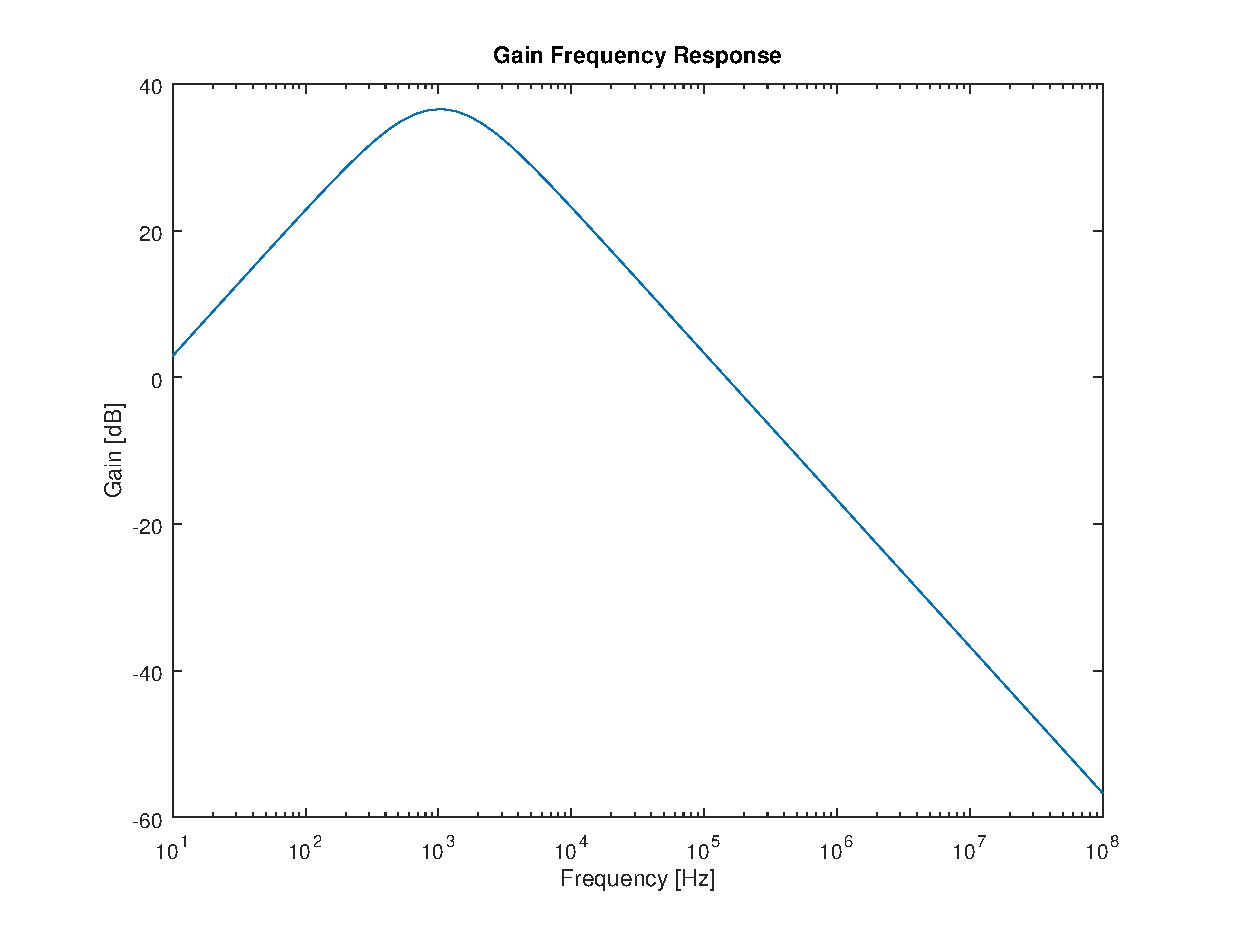
\includegraphics[scale=0.4]{theo_gain_f_response.eps}
    \caption{Theoretical Gain Response}
\end{subfigure}%
\begin{subfigure}{.5\textwidth}
    \centering
    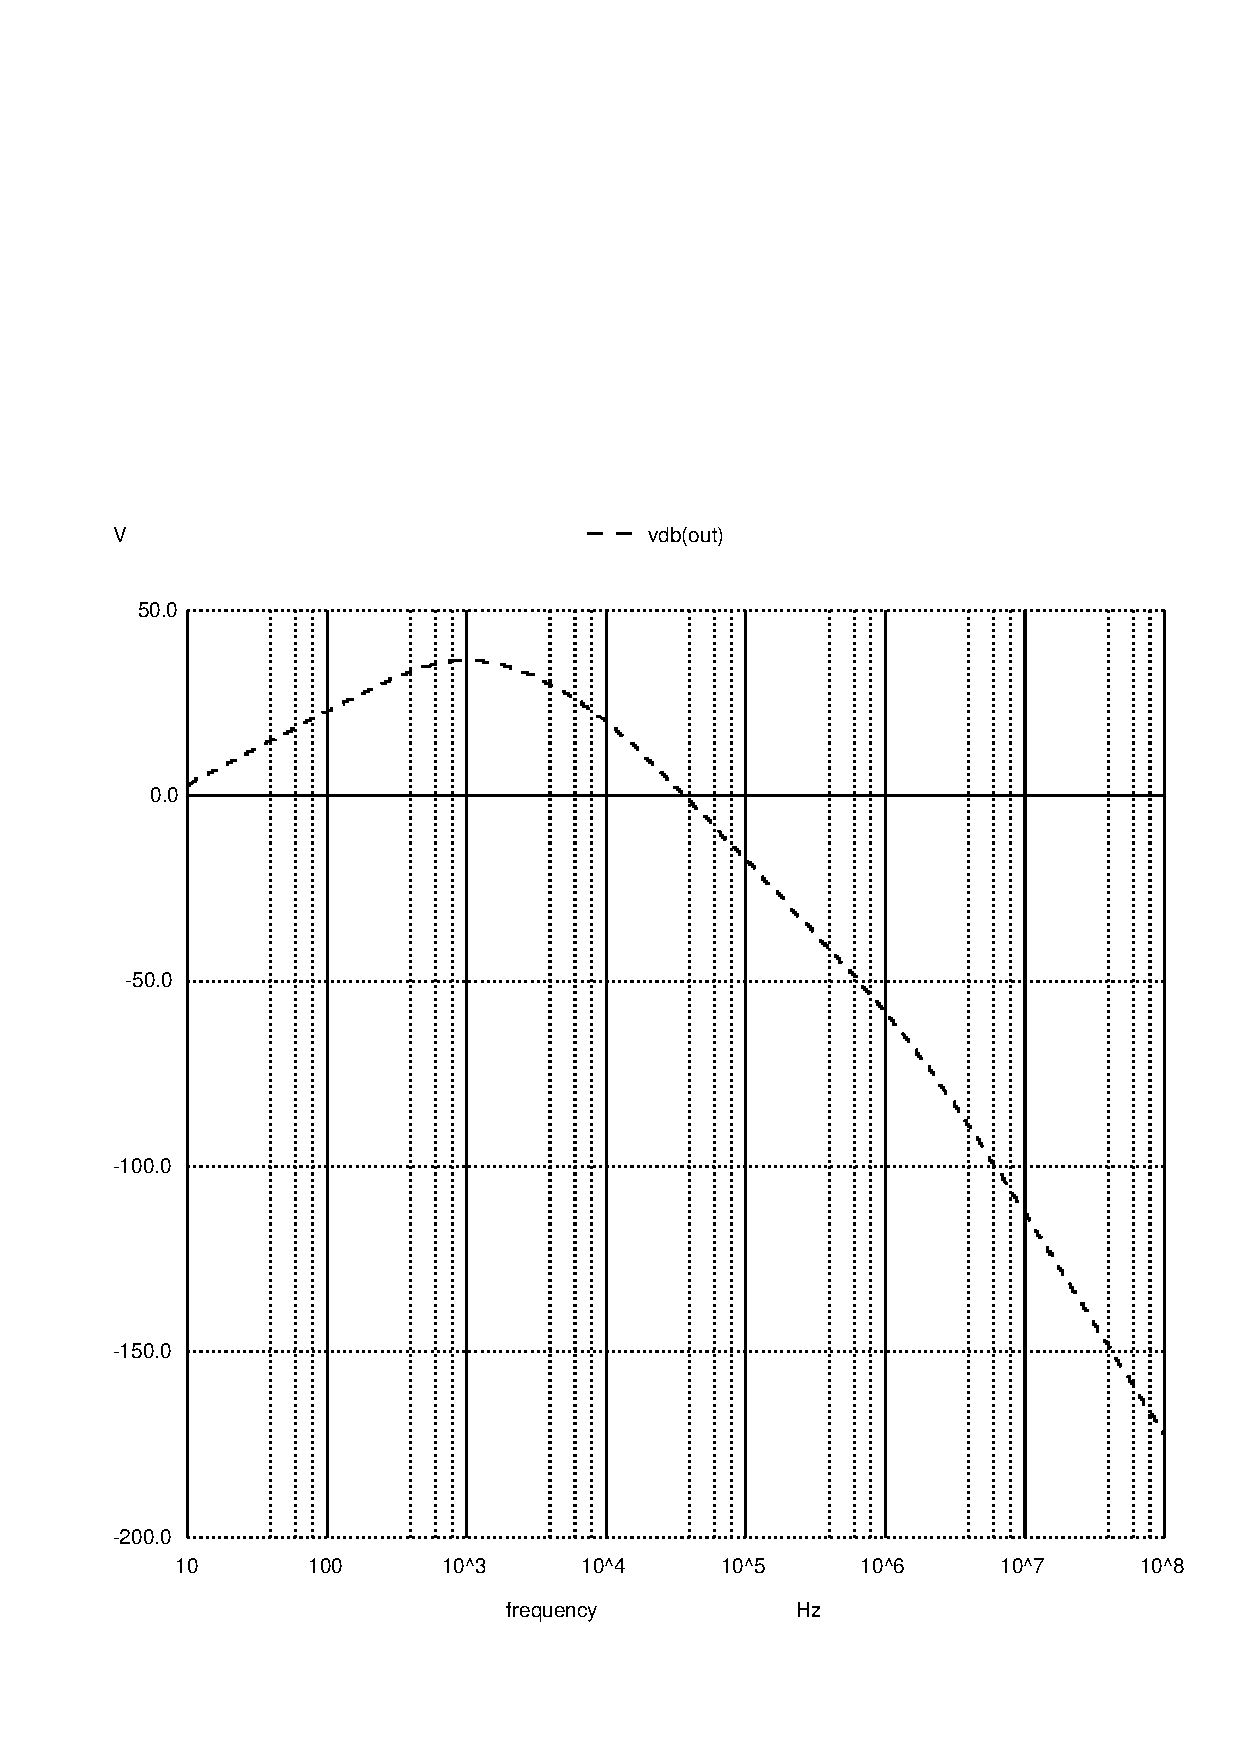
\includegraphics[scale=0.33]{vodb.pdf}
    \caption{Simulation Gain Response}
\end{subfigure}
\begin{subfigure}{.5\textwidth}
    \centering
    \vspace{2.8 cm}
    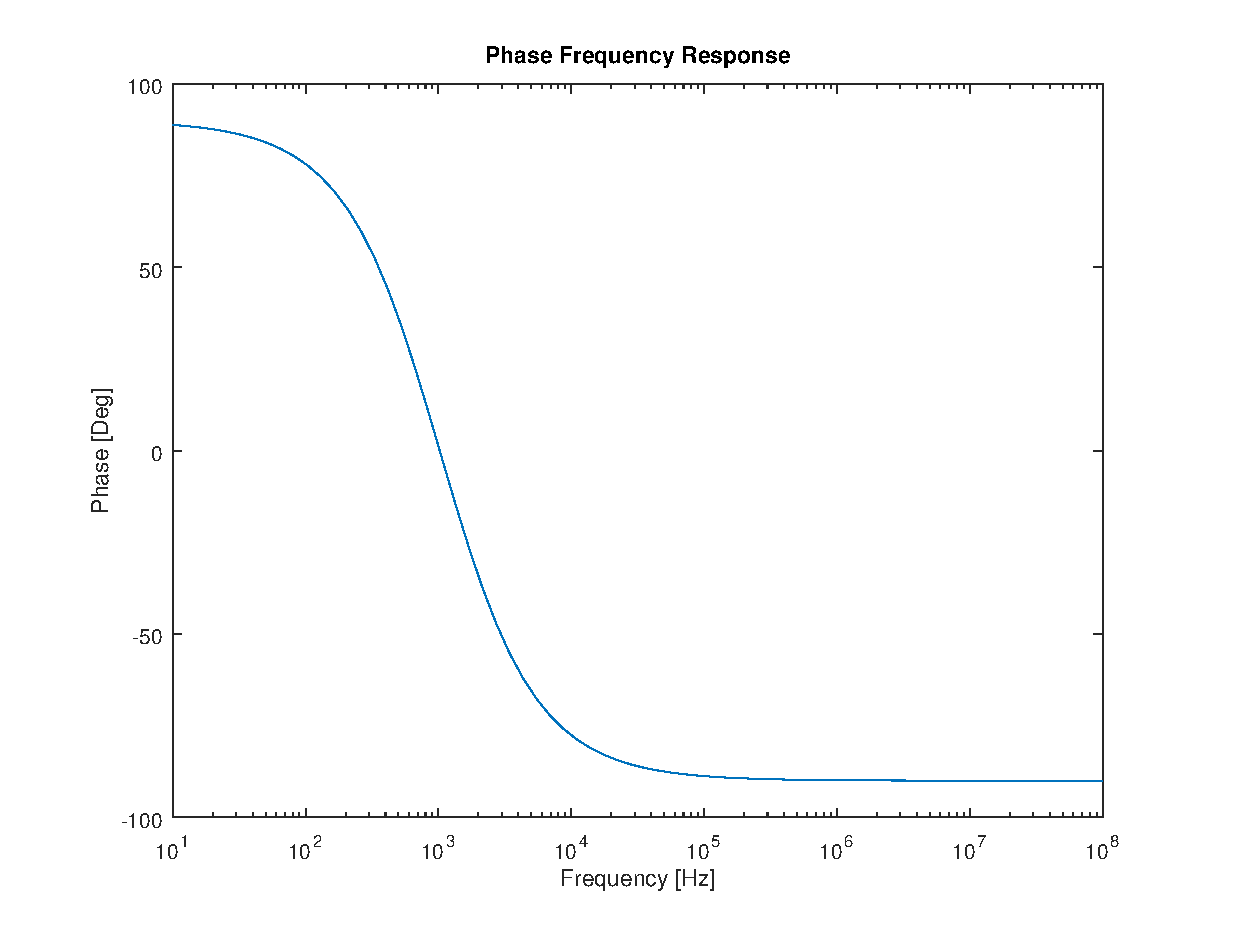
\includegraphics[scale=0.4]{theo_phase_f_response.eps}
    \caption{Theoretical Phase Response}
\end{subfigure}%
\begin{subfigure}{.5\textwidth}
    \centering
    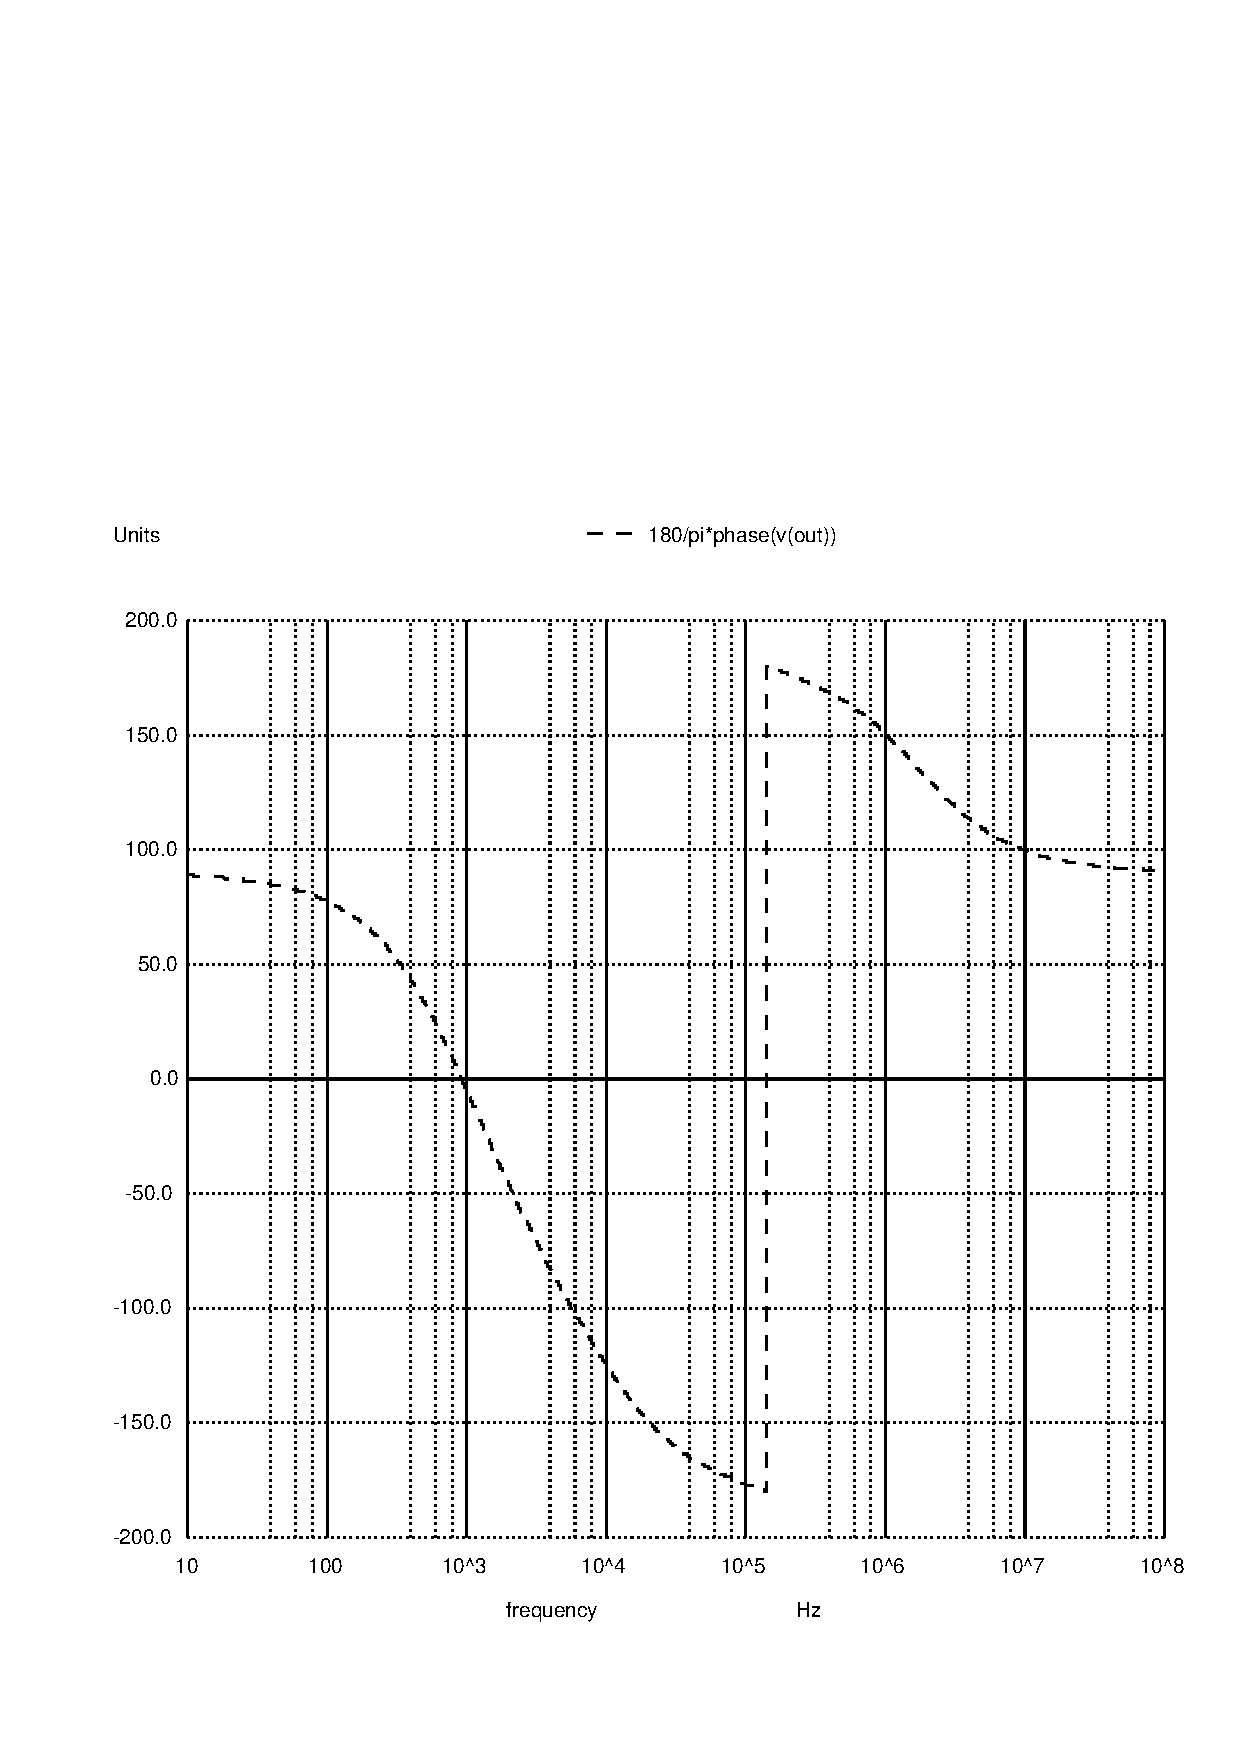
\includegraphics[scale=0.33]{voph.pdf}
    \caption{Simulation Phase Response}
\end{subfigure}
\caption{Frequency Response}
\label{fig:freq_resp}
\end{figure}

\clearpage

\section{Non-Improved Merit Results}
\label{sec:merit}

From the results obtained through the \textit{Ngspice} simulation (see Section \ref{subsec:comparison}) and considering we used the data shown in Section \ref{sec:introduction}, we can compute the price and the merit using the \textit{formulae} given in the lab assignment:

\begin{table}[h]
    \centering
    \begin{tabular}{|l|c|c|}
    \hline
    {\bf Name} & {\bf Value} & {\bf Units} \\ \hline
    AV dev & 32.9164 & \\ \hline
Freq dev & 13.911 & Hz\\ \hline
Cost & 13426.8 & MU\\ \hline
Merit & 1.59048E-06 & \\ \hline

   \end{tabular}
   \caption{Merit Results}
   \label{tab:merit}
\end{table}

\section{Circuit Improvements}
\label{sec:circuit_improvements}

Because some specifications of our circuit are a bit lacklustre, some additional improvements can be made. The main approach to improve the overall results was to increase the gain of the OPAMP stage. This was done by adding a bypass capacitor in series with resistor $R_4$. The expression of the gain is:

\begin{equation}
    A_v=1+\frac{Z_3}{Z_4}
\end{equation}

By adding the bypass capacitor, the impedance $Z_4$ decreases for high frequencies, and so the gain increases.

In order do adjust the low and high cut-off frequencies, some modifications were made to perfect these values, since the goal is that:

\begin{equation}
    f_o= \frac{\sqrt{w_H w_L}}{2\pi} = 1000 Hz
\end{equation}

These modifications were mainly the addition of resistors in series/parallel to increase/decrease the equivalent resistance seen and add, in the same way, capacitors in series/parallel in order to decrease/increase the overall capacity. This perfected both the gain at $1000 Hz$ as well as the low and high cut-off frequencies.   

\begin{figure}[h]
    \centering
    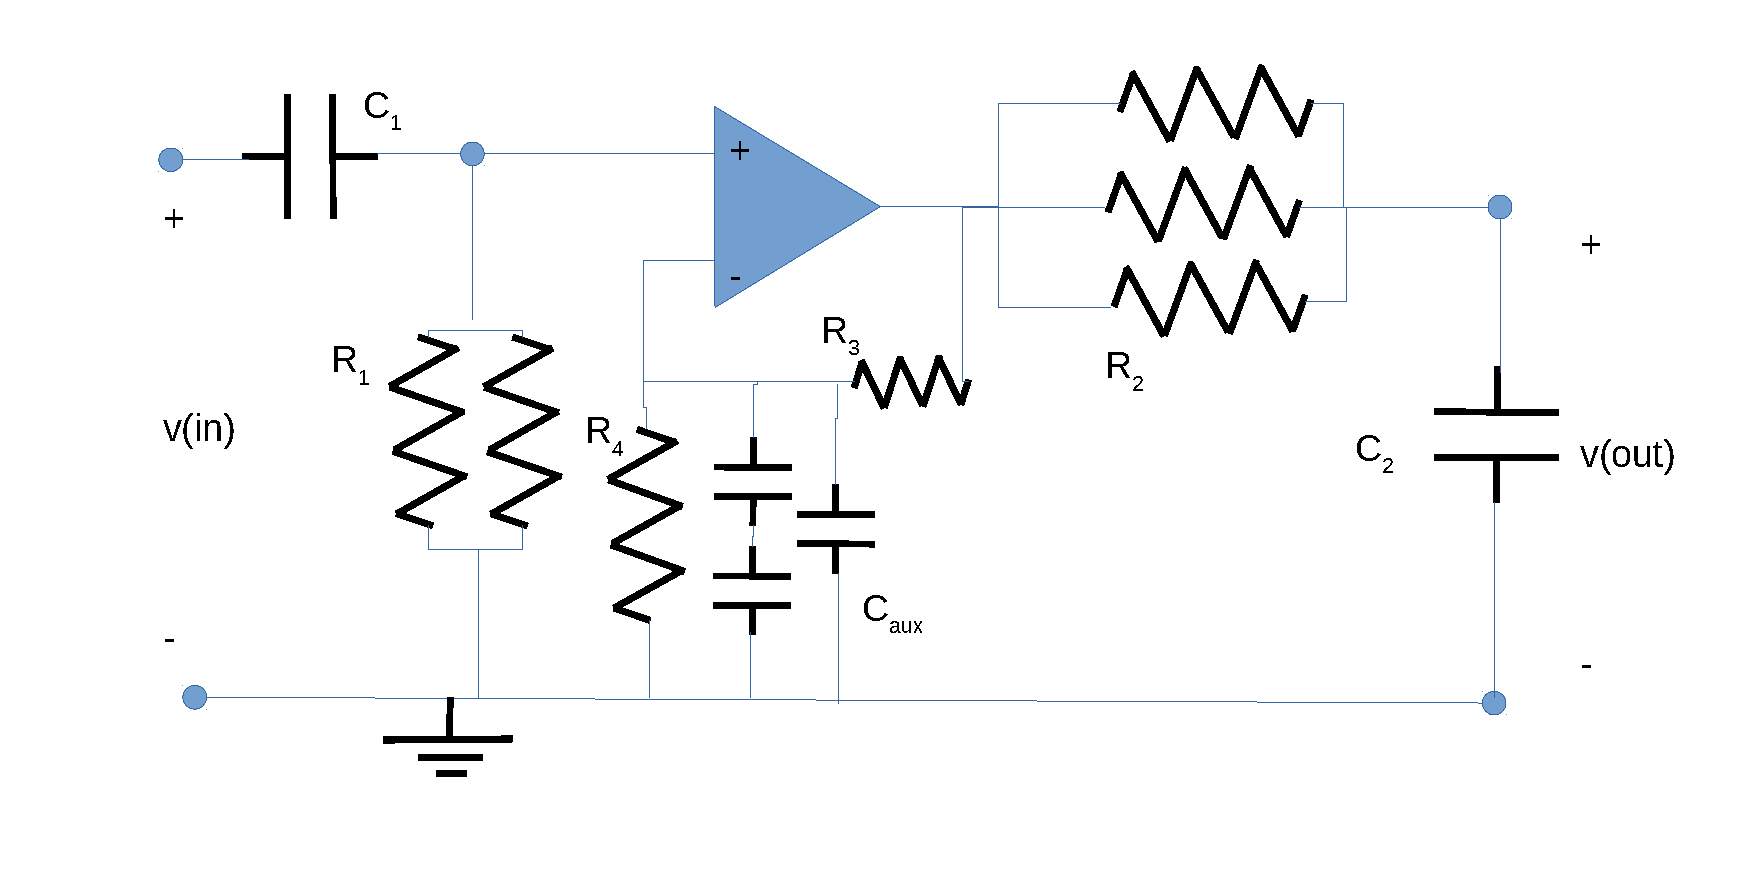
\includegraphics[scale=0.4]{circuitl5_new.pdf}
    \caption{Improved circuit}
    \label{fig:new_circuit}
\end{figure}

\clearpage

\begin{table}[h]
    \centering
    \begin{tabular}{|l|c|c|}
    \hline
    {\bf Name} & {\bf Value} & {\bf Units} \\ \hline
    $R_1$ & $500$ & $\Omega$ [Ohms] \\ \hline
    $R_2$ & $30000$ & $\Omega$ [Ohms] \\ \hline
    $R_3$ & $100000$ & $\Omega$ [Ohms] \\ \hline
    $R_4$ & $1000$ & $\Omega$ [Ohms] \\ \hline
    $C_1$ & $220$ & $\eta F$ [$\eta$Farads]\\ \hline
    $C_2$ & $220$ & $\eta F$ [$\eta$Farads] \\ \hline
    $C_{aux}$ & $1.5$ & $\mu F$ [$\mu$Farads]\\ \hline
    \end{tabular}
    \caption[Constants Values for the improved circuit]{Constants Values \footnotemark for the improved circuit}
    \label{tab:constants_new}
\end{table}
\footnotetext{Note that these values reflect and summarise the composition shown in Figure \ref{fig:new_circuit} and, as so, some components may actually reflect a certain composition of multiple ones.}
The results that come from these modifications are shown below:

\begin{table}[h]
    \centering
    \begin{tabular}{|l|c|c|}
    \hline
    {\bf Name} & {\bf Value} & {\bf Units} \\ \hline
    AV & 40.7735 & dB\\ \hline
fO & 1028.02 & Hz\\ \hline

    \end{tabular}
    \caption[Improved Results]{Improved Results \footnotemark}
    \label{tab:results_new}
\end{table}
\footnotetext{Gain is measured at a frequency of 1000Hz.}
\vspace{-3 cm}
\begin{figure}[h]
    \centering
    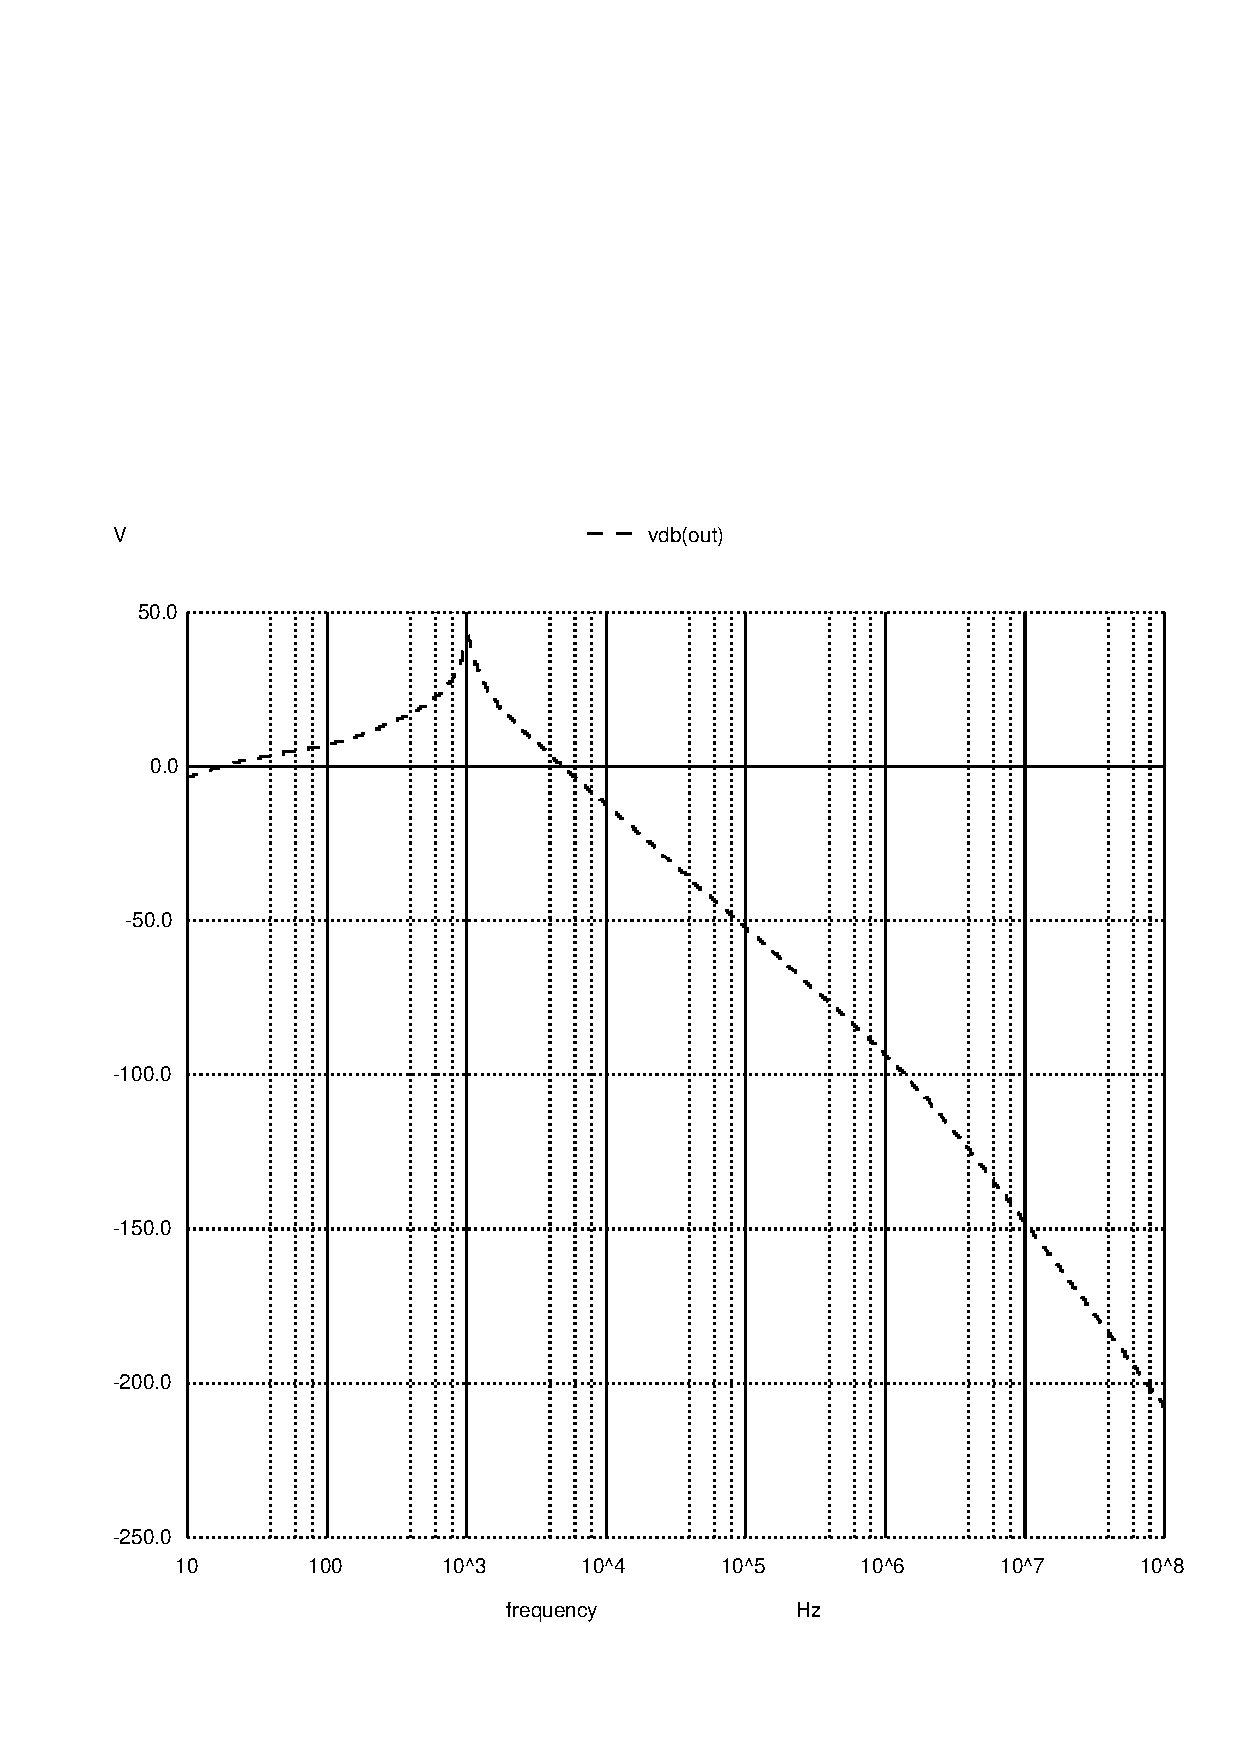
\includegraphics[scale=0.33]{vodb_new.pdf}
    \caption{Gain Frequency Response}
    \label{fig:gain_resp_new}
\end{figure}

\begin{table}[h]
    \centering
    \begin{tabular}{|l|c|c|}
    \hline
    {\bf Name} & {\bf Value [$\Omega$]}  \\ \hline
    Input Imp & 500.706 + -725.317 j\\ \hline

    Output Imp & 17.5248 + -723.225 j\\ \hline

    \end{tabular}
    \caption{Input and Output Impedances}
    \label{tab:imp_new}
\end{table}

With these changes, we managed to decrease massively the output impedance. With this configuration, the circuit is much more prepared to be connected to a greater range of loads, which increases its utility in practical terms. Another plus are the better results, as shown in table \ref{tab:results_new}, when compared to the ones previously obtained (in table \ref{tab:exp_gain_freq}).

\pagebreak

\section{Improved Merit Results}
\label{sec:merit_new}

\begin{table}[h]
    \centering
    \begin{tabular}{|l|c|c|}
    \hline
    {\bf Name} & {\bf Value} & {Units}\\ \hline
    AV dev & 9.31408 & \\ \hline
Freq dev & 28.016 & Hz\\ \hline
Cost & 13459.5 & MU\\ \hline
Merit & 1.99026E-06 & \\ \hline

    \end{tabular}
    \caption{Improved Merit Results}
    \label{tab:merit_new}
\end{table}

With the improvements made, even though the central frequency was slightly worse, the benefit of the increase in the gain excelled making the merit figure rise, giving us the results shown in table \ref{tab:merit_new}.





\section{Conclusion}
\label{sec:conclusion}

As a conclusion, we can state that, unlike the previous two lab assignments, there is a degree of similarity between both analysis, in terms of precision. This was rather surprising, for we are dealing with a high-complexity component - the OPAMP - at least in terms of architecture. But, when we analyse it in a macroscopical point of view, it's rather predictable and stable - at least in this circuit. 

Overall, the laboratory gave us the opportunity to deepen our knowledge with OPAMPs and Active 2nd-order filters. We understood it as an extension of the second lab, where we analysed 1st-order RC circuits. 

It is also worth noting that the concept of the merit figure proves itself to be extremely important, because it narrows the gap between an academic point of view and an industrial/engineering approach. It made us understand that there are many factors involved in the construction of a circuit, some of them being the cost, the space availability and the customers' needs. Another limiting factor was the fixed values and quantities for each of the components, which made us have to think more thoroughly and inventively about how and where we would use them. A complete circuit that takes into account all these factors is most of the times really hard to achieve, which leads us to sacrifice some characteristics in favour of some more important others, achieving a balance between them all.


%\cleardoublepage

% ----------------------------------------------------------------------
%  Bibliography
% ----------------------------------------------------------------------
%\addcontentsline{toc}{section}{\bibname}
%\bibliographystyle{abbrvunsrtnat} % <<<<< SELECT IF USING REFERENCES BY NUMBER (CITATION ORDER)
%\bibliography{../../../BIBfile.bib}

% ----------------------------------------------------------------------
\end{document}
% ----------------------------------------------------------------------

